\documentclass[11pt,a4paper]{article}
\usepackage[T2A,T1]{fontenc}
\usepackage[utf8]{inputenc}
\usepackage[english,russian]{babel}
\usepackage{geometry}
\usepackage{graphicx}
\usepackage{booktabs}
\usepackage{microtype}
\usepackage[hidelinks]{hyperref}
\geometry{margin=18mm}
\graphicspath{{results_tau1_no_gap/}}
\setlength{\parindent}{1.1em}
\setlength{\parskip}{0.25em}
\hypersetup{
  pdftitle={EDM-анализ резкой генерализации без memorization gap},
  pdfauthor={2026-Project-202},
  pdfsubject={EDM-анализ training-log.csv при tau=1},
  pdfkeywords={EDM, grokking, intrinsic dimension, MLE, FNN, Cao, simplex}
}
\newcommand{\code}[1]{{\fontencoding{T1}\selectfont\ttfamily #1}}

\title{EDM-анализ резкой генерализации\\без memorization gap}
\author{Контрольный эксперимент на $S_n$}
\date{1 августа 2026 г.}

\begin{document}
\maketitle

\begin{abstract}
Проведён скользящий EDM-анализ запуска, в котором train- и validation-accuracy
растут практически синхронно. Использованы четыре проектных метода оценки
размерности: False Nearest Neighbors, Cao, simplex projection и
Levina--Bickel MLE при фиксированной задержке $\tau=1$. Резкая генерализация
сопровождается выраженной перестройкой локальной геометрии временных рядов, но
не единым dimensionality collapse: MLE validation loss снижается, тогда как
MLE общей gradient norm устойчиво растёт. Результат поддерживает трактовку EDM
как маркера смены режима оптимизационной динамики, а не как универсального
скалярного порядка grokking.
\end{abstract}

\section{Данные и положение перехода}

Файл \code{training\_log.csv} содержит 2221 наблюдение, записанное каждые
20 optimizer steps, и охватывает шаги 0--44400. В отличие от классического
grokking, длительного интервала между запоминанием train-set и обобщением нет.

\begin{table}[ht]
\centering
\caption{Устойчивые пороги accuracy: пять последовательных лог-точек.}
\begin{tabular}{lr}
\toprule
Событие & Шаг \\
\midrule
Validation accuracy $\ge 0.50$ & 43420 \\
Validation accuracy $\ge 0.90$ & 44040 \\
Batch train accuracy $\ge 0.95$ & 44160 \\
Validation accuracy $\ge 0.95$ & 44300 \\
\bottomrule
\end{tabular}
\end{table}

Validation accuracy достигает 0.90 на 120 шагов раньше, чем batch train
accuracy устойчиво достигает 0.95. Поэтому наблюдается резкий совместный
переход обучения и генерализации, а не memorization plateau с последующим
grokking.

\begin{figure}[ht]
\centering
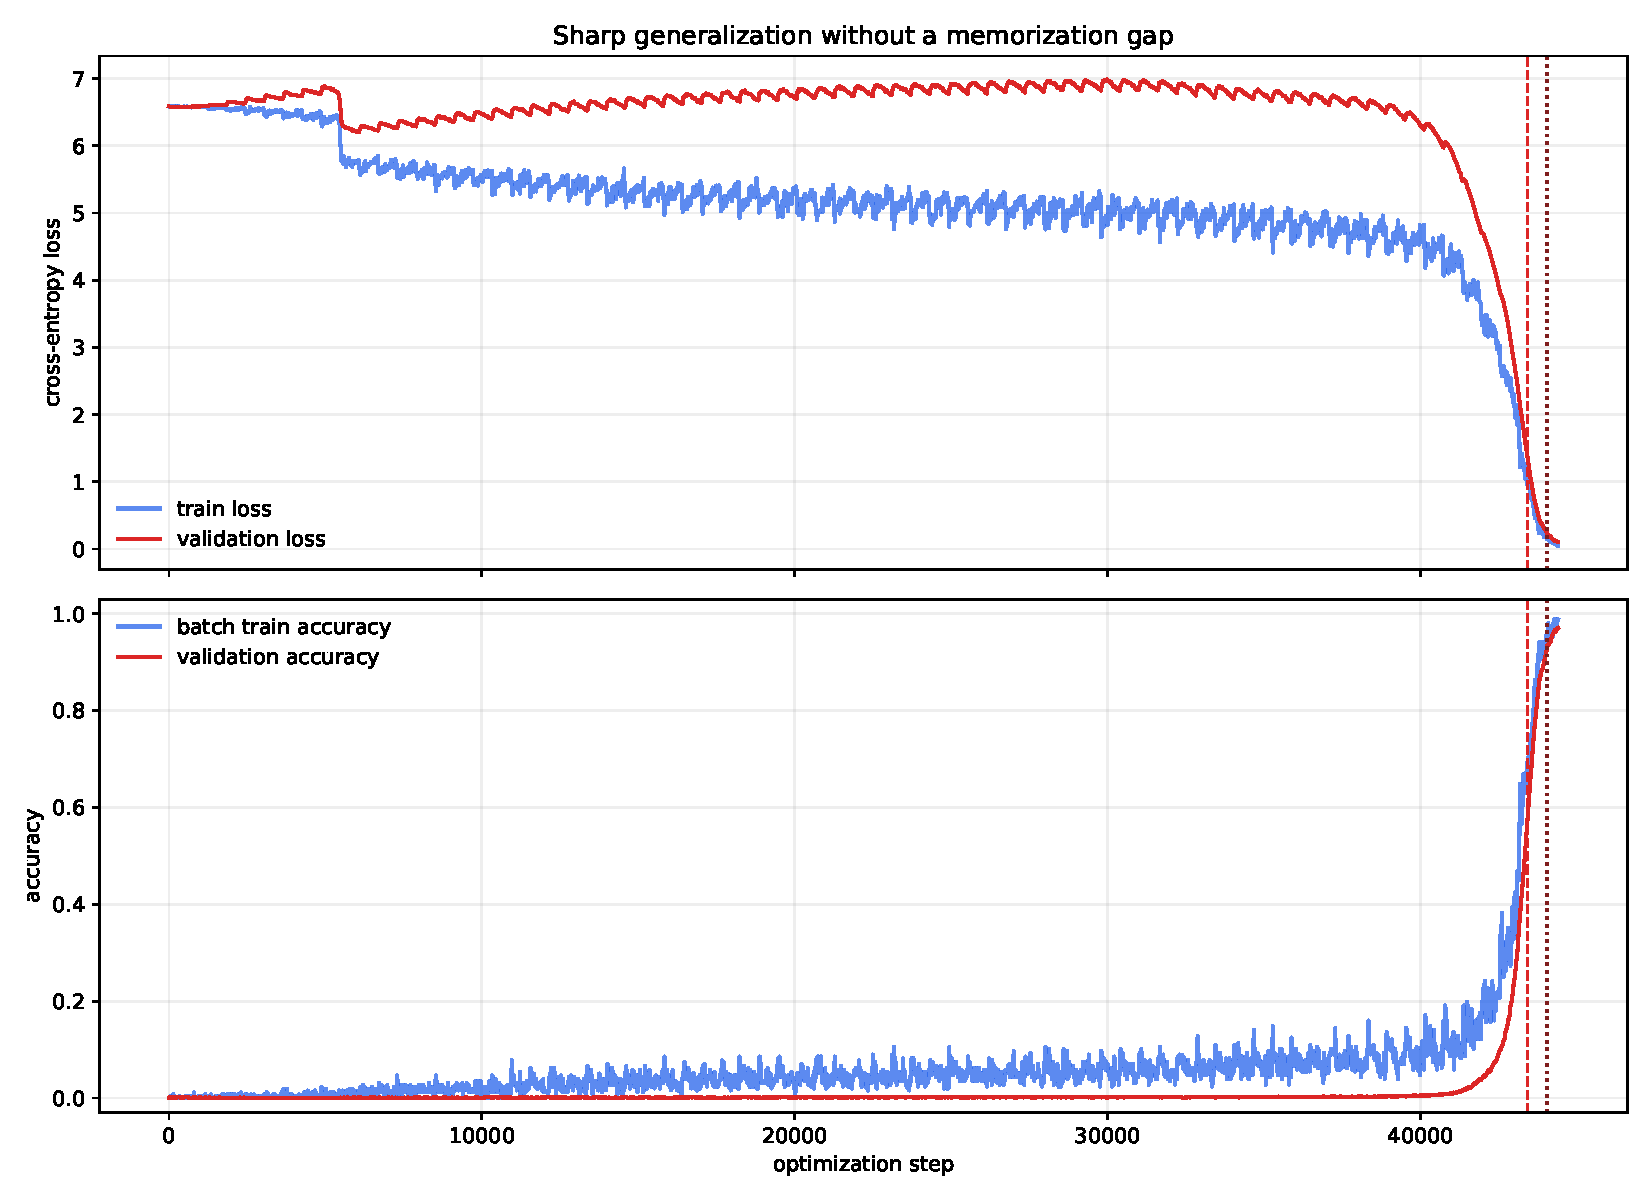
\includegraphics[width=\textwidth]{01_training_transition.pdf}
\caption{Train/validation loss и accuracy. Красный пунктир --- устойчивое
достижение validation accuracy 0.50, точечная линия --- достижение 0.90.}
\end{figure}

\clearpage
\section{Методика EDM}

Основной анализ выполнен со следующими настройками:

\begin{itemize}
\item фиксированная задержка $\tau=1$;
\item окно 100 лог-точек, то есть 2000 optimizer steps;
\item stride 10 лог-точек, то есть 200 optimizer steps;
\item максимальная embedding dimension $E_{max}=15$;
\item пять соседей для Levina--Bickel MLE;
\item исходные и локально линейно detrended временные ряды.
\end{itemize}

Анализируются \code{train\_loss}, \code{val\_loss}, \code{weight\_norm},
\code{grad\_norm}, \code{embed\_grad\_norm} и \code{grad\_cosine}. Для
MLE дополнительно проверены окна 50 и 150 точек.

После устойчивого достижения validation accuracy 0.95 остаётся только шесть
лог-точек. Поэтому отдельная post-transition фазовая реконструкция невозможна:
последние пять окон смешивают подход к переходу и сам переход. Они сравниваются
с последними пятью полностью пред-переходными окнами, заканчивающимися до
шага 42500.

\section{Четыре метода на loss}

\begin{figure}[ht]
\centering
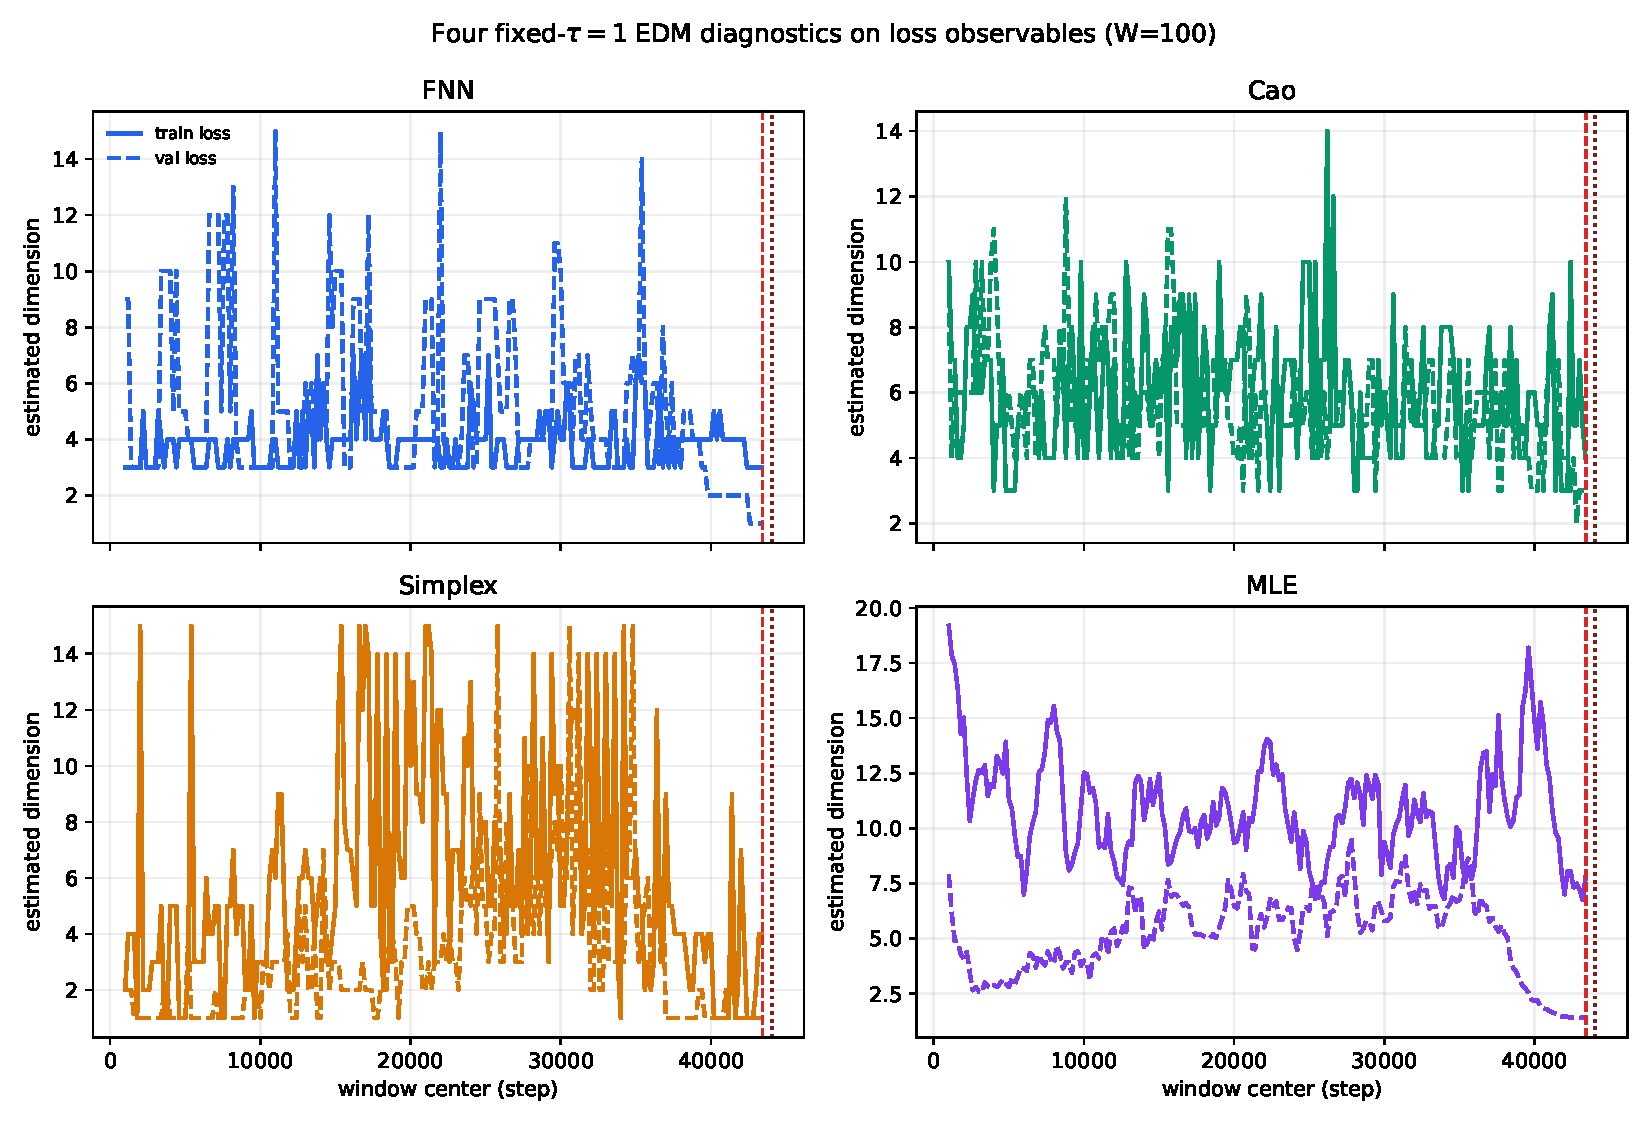
\includegraphics[width=\textwidth]{02_four_methods_loss.pdf}
\caption{FNN, Cao, simplex и MLE на train- и validation-loss.}
\end{figure}

\begin{table}[ht]
\centering
\small
\caption{Transition-window mean минус pre-transition mean.}
\begin{tabular}{llrr}
\toprule
Метрика & Метод & Raw $\Delta$ & Detrended $\Delta$ \\
\midrule
Train loss & FNN     & -1.20 & -0.40 \\
Train loss & Cao     & -0.80 & +0.40 \\
Train loss & Simplex & -0.20 & +1.60 \\
Train loss & MLE     & -4.78 & -0.77 \\
\midrule
Validation loss & FNN     & -1.00 & -0.80 \\
Validation loss & Cao     & -2.60 & -0.80 \\
Validation loss & Simplex & -0.20 & +0.20 \\
Validation loss & MLE     & -0.30 & -1.65 \\
\bottomrule
\end{tabular}
\end{table}

Raw MLE train loss резко падает с 12.09 до 7.31, но после удаления локального
линейного тренда изменение уменьшается с $-4.78$ до $-0.77$. Значительная
часть raw-сигнала, следовательно, создаётся формой быстрого падения loss.
Для validation loss падение detrended MLE остаётся выраженным.

\clearpage
\section{MLE по всем наблюдаемым}

\begin{figure}[ht]
\centering
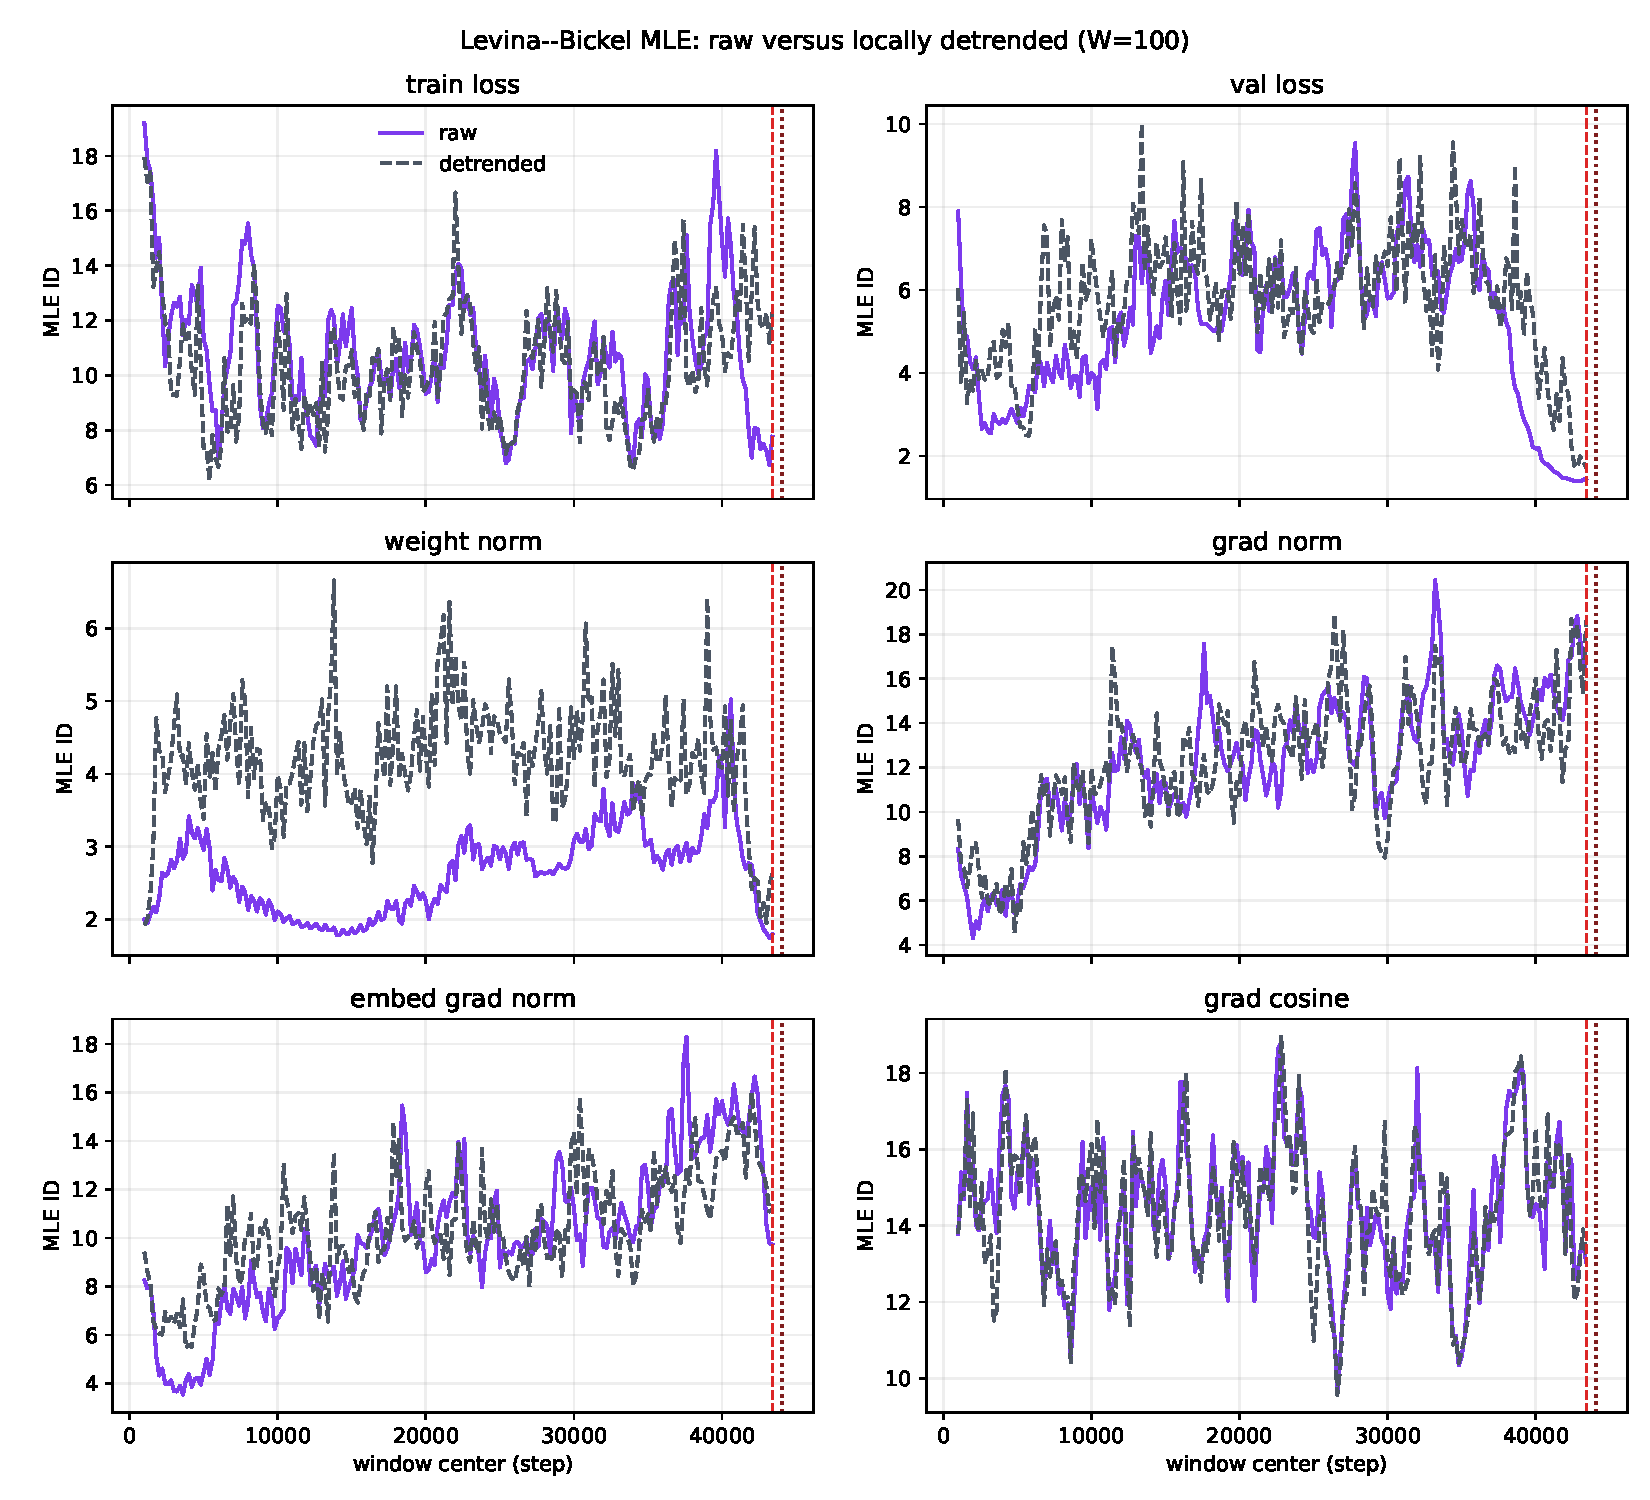
\includegraphics[width=\textwidth]{03_mle_all_metrics.pdf}
\caption{Levina--Bickel MLE исходных и локально detrended рядов.}
\end{figure}

\begin{table}[ht]
\centering
\small
\caption{Средние пяти пред-переходных и пяти переходных окон, $W=100$.}
\begin{tabular}{lrrrr}
\toprule
& \multicolumn{2}{c}{Raw MLE} & \multicolumn{2}{c}{Detrended MLE} \\
Метрика & Pre & Transition & Pre & Transition \\
\midrule
Train loss              & 12.09 & 7.31  & 12.64 & 11.87 \\
Validation loss         & 1.72  & 1.42  & 3.46  & 1.81 \\
Weight norm             & 3.64  & 1.84  & 4.36  & 2.26 \\
Gradient norm           & 15.58 & 17.61 & 14.41 & 17.37 \\
Embedding-gradient norm & 15.16 & 11.36 & 14.63 & 12.01 \\
Gradient cosine         & 14.97 & 13.04 & 15.54 & 12.92 \\
\bottomrule
\end{tabular}
\end{table}

Наиболее важное несогласие наблюдаемых --- противоположный знак gradient norm.
Её detrended MLE увеличивается примерно на 2.96, хотя validation loss и
несколько других рядов упрощаются. Следовательно, переход не является
глобальным сжатием всей оптимизационной динамики.

\begin{figure}[ht]
\centering
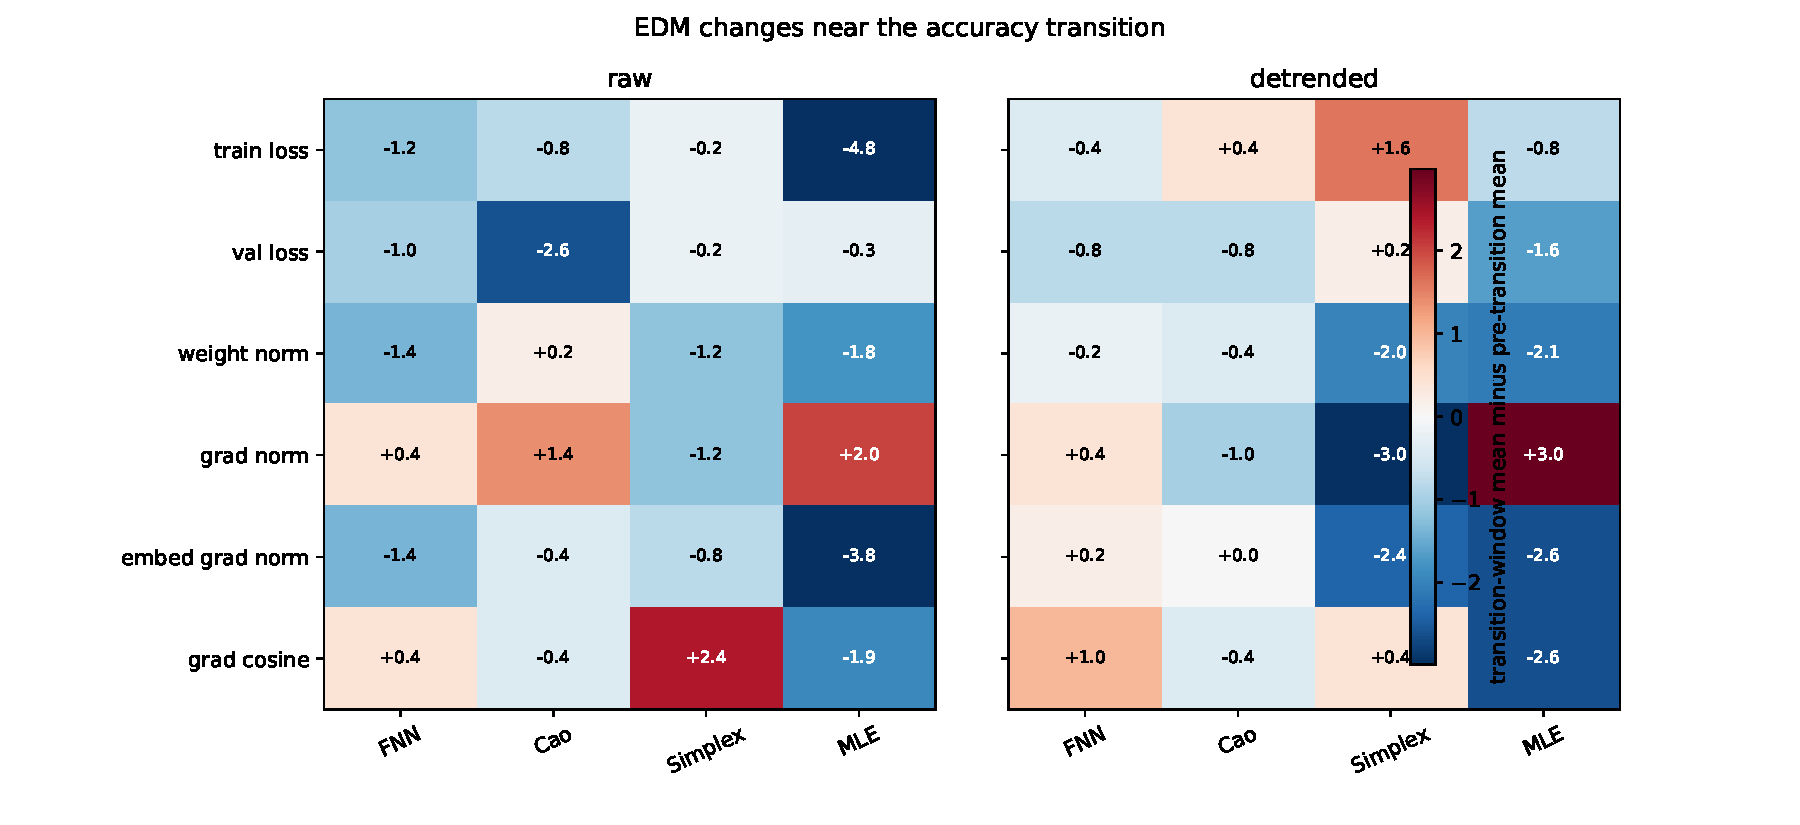
\includegraphics[width=0.92\textwidth]{04_method_delta_heatmap.pdf}
\caption{Изменения всех четырёх методов у перехода. Синий цвет означает
снижение оценки, красный --- рост.}
\end{figure}

\clearpage
\section{Чувствительность к длине окна}

\begin{figure}[ht]
\centering
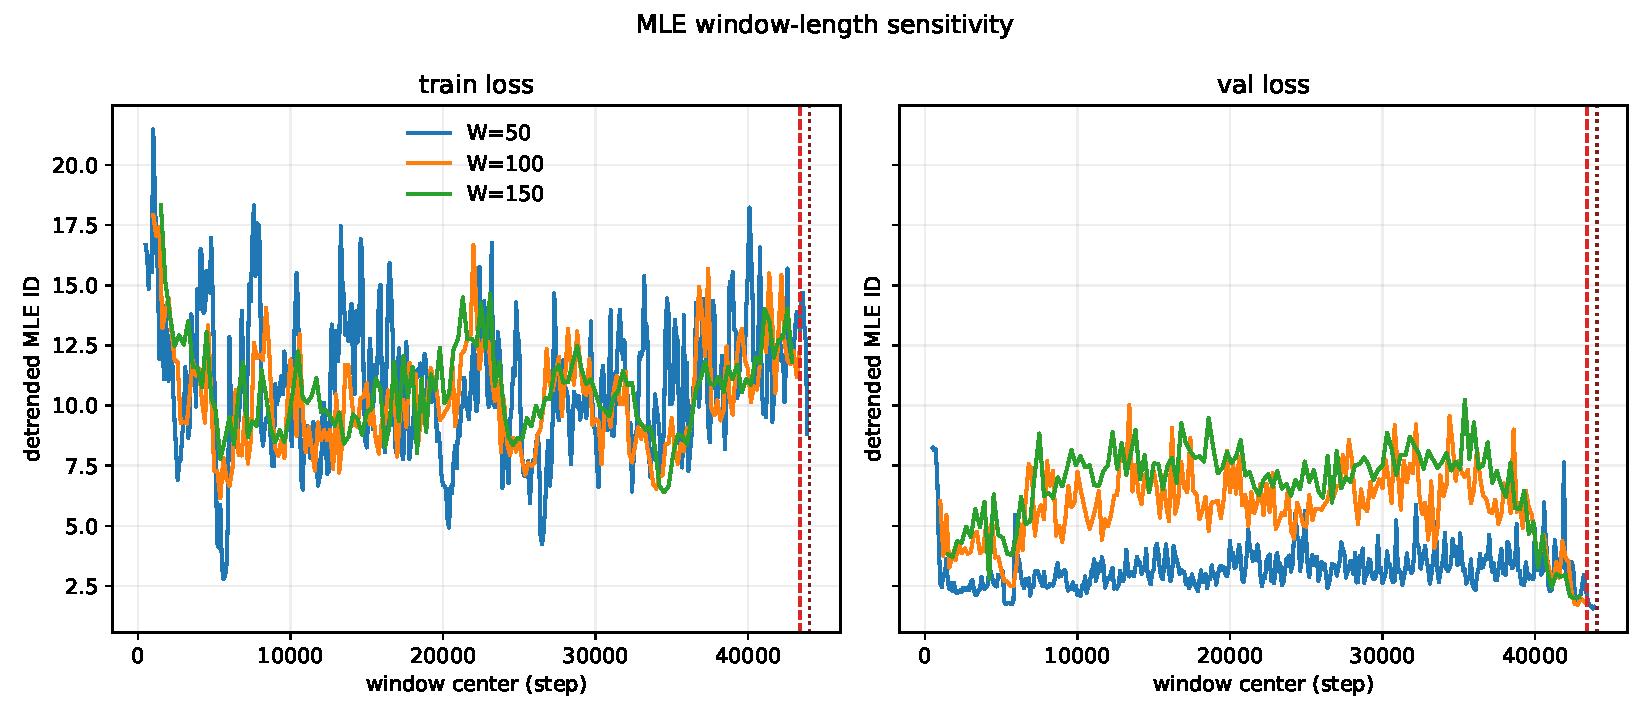
\includegraphics[width=\textwidth]{05_mle_window_robustness.pdf}
\caption{Detrended MLE loss при окнах 50, 100 и 150 лог-точек.}
\end{figure}

\begin{table}[ht]
\centering
\small
\caption{Detrended MLE: transition минус pre-transition.}
\begin{tabular}{lrrrc}
\toprule
Метрика & $W=50$ & $W=100$ & $W=150$ & Устойчивый знак \\
\midrule
Validation loss         & -2.65 & -1.65 & -1.78 & да \\
Gradient norm           & +5.51 & +2.96 & +2.30 & да \\
Train loss              & +1.87 & -0.77 & +1.42 & нет \\
Weight norm             & +1.09 & -2.09 & -2.64 & нет \\
Embedding-gradient norm & -1.89 & -2.62 & -0.58 & да \\
Gradient cosine         & -3.36 & -2.62 & +0.43 & нет \\
\bottomrule
\end{tabular}
\end{table}

Наиболее устойчивы два противоположных эффекта: снижение MLE validation-loss
траектории и увеличение MLE gradient-norm траектории. Падение train-loss MLE
после detrending не устойчиво к длине окна.

\section{Ограничения}

\begin{enumerate}
\item После перехода недостаточно наблюдений для независимой post-transition
фазы.
\item Окна перекрываются на 90\% и не являются статистическими повторениями.
\item Legacy nearest-neighbour методы не используют Theiler exclusion.
\item 141 raw и 113 detrended MLE-оценок превышают $E_{max}=15$; максимумы
равны 20.44 и 18.94. Это выход legacy-эвристики, а не буквальная размерность
15-мерного embedding.
\item Simplex выбирает верхнюю границу $E=15$ примерно в 16.4\% raw окон
gradient cosine, но значительно реже для остальных наблюдаемых.
\item Имеется один запуск и один seed, поэтому вывод является описательным.
\end{enumerate}

\section{Вывод}

Резкое обобщение без memorization gap сопровождается измеримой EDM-перестройкой.
Однако её направление зависит от observable и метода. Validation-loss динамика
становится более низкоразмерной, тогда как динамика общей нормы градиента
становится более сложной. Поэтому EDM в этом эксперименте является маркером
смены режима оптимизации, но не подтверждает универсальный dimensionality
collapse всей системы.

\paragraph{Воспроизводимость.}
Полные таблицы находятся в \code{results\_tau1\_no\_gap/}; скрипт расчёта ---
\code{analyze\_sharp\_no\_gap\_edm.py}.

\end{document}
